\section{Convolution}

The \emph{convolution} of a signal $x$ with a signal $h$ is given by
\begin{align}
    x(t) * h(t) & = \int_{-\infty}^{\infty} x(\tau) h(t - \tau) d\tau \\
    x[n] * h[n] & = \sum_{k=-\infty}^{\infty} x[k] h[n - k].
\end{align}
Graphically, we can envision this as flipping $h$ and sliding it
along the horizontal axis, finding and summing the area of $h$
times $x$ as we slide $h$ along. $x$ remains stationary, so the
bounds of the integral (or summation in the discrete case) are determined
by the window of overlap between $x$ and the flipped $h$
(see figure \ref{fig:convolution}).

\begin{figure}[h]
    \centering
    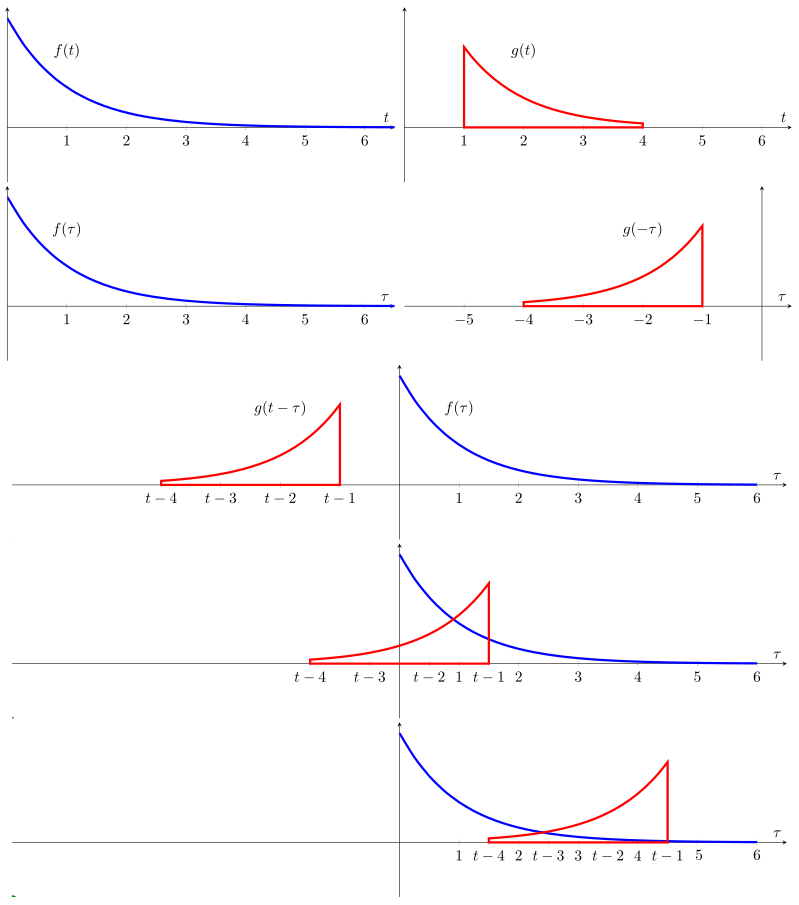
\includegraphics{images/Convolution3.svg.png}
    \caption{Convolution}
    \label{fig:convolution}
\end{figure}



This definition may seem arbitrary at first, but convolution has
incredibly useful properties in signal analysis. For instance, an
LTI system is completely characterized by its impulse response $h$,
the value obtained by plugging in $\delta$ to the system, with
$y = x * h$.

Recall the sifting property of the unit impulse,
\begin{align}
    x(t) = \int_{-\infty}^{\infty} x[\tau] \delta[\tau - t] d\tau \\
    x[n] = \sum_{k=-\infty}^{\infty} x[k] \delta[n - k]
\end{align}

This property is useful in that it allows us to represent
$x(t)$ or $x[n]$ as a series of scaled very simple functions. It also
tells us that $x$ convolved with $\delta$ yields $x$.

Convolution has the following properties:
\begin{itemize}
    \item Commutativity: $x_1(t) * x_2(t) = x_2(t) * x_1(t)$
    \item Distributivity over addition:
          $x_1(t) * (x_2(t) + x_3(t)) = x_1(t)*x_2(t) + x_1(t)*x_3(t)$
    \item Associative: $x_1(t) * (x_2(t) * x_3(t)) = (x_1(t) * x_2(t)) * x_3(t)$
\end{itemize}